%Obviously, the waiting cost of synchronous aggregation is sometime harmful, So we proposed using asynchronous aggregation to reduce the coordination.
%In this section, we first formally define asynchronous aggregation and introduce accumulated recursive aggregation program. We then propose the sufficient conditions for returning correct results by analyzing the aggregate/non-aggregate operations.And then we propose a conversion technology for some unsatisfied algorithm.
%In this section, we propose the foundations of automatic asynchronous aggregation.


\section{Asynchronous Recursive Aggregation}

To support asynchronous processing and integrate the advantage of semi-naive evaluation, we first propose a special form of recursive aggregation, named accumulated recursive aggregation. Then we give the formal definition of asynchronous aggregation. Finally, we provide the sufficient conditions for correct asynchronous aggregation.

\subsection{Accumulated Recursive Aggregation}
\label{sec:async:accrec}

{
%\begin{comment}
	\begin{figure}[t]
		\vspace{-0.1in}
		\centerline{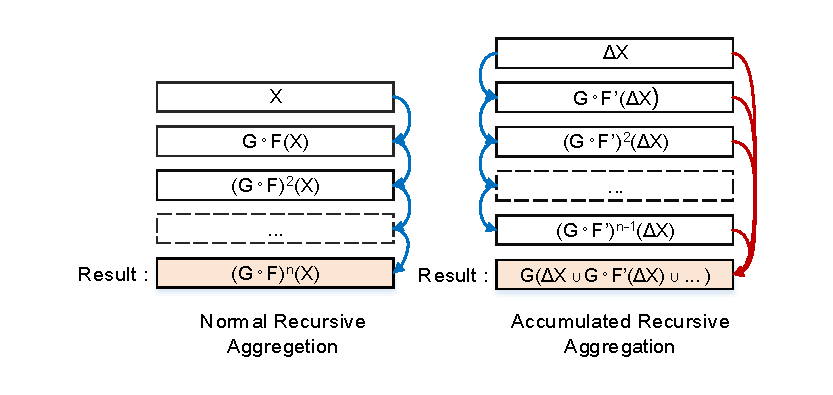
\includegraphics[width=4in]{fig/accumulative.pdf}}
		\caption{Normal Recursive Aggregation and Accumulated Recursive Aggregation }
		\vspace{-0.1in}
		\label{fig:arasssp}
	\end{figure}
%\end{comment}	

We observed that some of the Recursive aggregation has the potential to be evaluated incrementally, when monotonic conditions are satisfied. i.e., The result of the previous recursion needs to involved in the next recursion. Take SSSP as example, the $\$min$ operation takes both newly generated paths and the current minimum distance as input to find the minimum distance. We find that these program can be rewrite as accumulated recursive aggregation forms that has the potential to asynchronouly processing e.q., figure \ref{fig:arasssp}. Hence we gives the definition and constraint of accumulated recursive aggregation.


\begin{definition}
	\label{th:monotone}
	(\textbf{Accumulated Asynchronous}) 
	\begin{itemize}
		\item \textbf{communitive}: $G(Y_1\cup Y_2)=G(Y_2\cup Y_1)$
		\item \textbf{monotonic}: $X\subseteq F(X)$
		\item \textbf{accumulative}: $G(Y_1\cup Y_2)=G(G(Y_1)\cup Y_2)$
		\item \textbf{idempotent}: $G(Y_1\cup Y_1)=G(Y_1)$
		\item \textbf{order-independent}: $G\circ F\circ G(X)=G\circ F(X)$
	\end{itemize}
	A normal recursive aggregate form can be converted to accumulated recursive aggregations, if the aggregate operation $G$ is communitive and accumulative and idempotent and non-aggregate operations $F$ is monotonic. And further the Order-independent property is satisfied.
\end{definition}
	
	\textbf{Accumulated Recursive Aggregation.} If a normal recursive aggregation  as defined with equation \ref{eq:recursive2} is accumulable, and make $F'(X)=F(X)-X$,  the accumulated recursive aggregation form can be represented as follows.
	\begin{equation}\label{eq:accumasync}
	\begin{aligned}
	\Delta Y^{k}&= F'(\Delta X^k)\\
	\Delta X^{k+1}&= G(\Delta Y^{k})\\
	X^{n}&=G(\cup_{i=0}^{n-1} \Delta Y^{i}\Delta X^0)
	\end{aligned}
	\end{equation}
	It starts from $\Delta X^0=X^0$ and terminates when there is no new $\Delta Y^k$ produced. The final result is the aggregation of all intermediate results. We can easily proof that the accumulated recursive aggregation return the same result with normal recursive aggregation as equation \ref{eq:recursive2}.
	

\begin{comment}
	\begin{align}
	&G( \Delta Y^0\cup F\circ G(\Delta Y^0)\cup\ldots)\notag \\
	=&G(G(F(\Delta X^0))\cup F\circ G(\Delta Y^0)\cup \ldots )\notag\\
	=&G\Big(F\circ G(\Delta Y^0)\cup (F\circ G)^2(\Delta Y^0)\cup \ldots ) \notag\\
	=& \ldots \notag \\
	=&G\Big((F\circ G)^k(\Delta Y^0)\Big)\notag\\
	=&(G \circ F)^{k+1}(X^0)\notag
	\end{align}
\end{comment}
{\color{yellow}
	\small
\begin{align}
&G( \ldots\cup (F'\circ G)^{k-2}(\Delta Y^0)\cup(F'\circ G)^{k-1}(\Delta Y^0))\notag \\
=&G( \ldots\cup G(F'\circ G)^{k-2}(\Delta Y^0)\cup(F'\circ G)(F'\circ G)^{k-2}(\Delta Y^0))\notag\\
=&G( \ldots\cup (F'\circ G)^{k-3}(\Delta Y^0)\cup(F\circ G)(F'\circ G)^{k-2}(\Delta Y^0))\notag\\
=& \ldots \notag \\
=&G\Big((F\circ G)^k(\Delta Y^0)\Big)\notag\\
=&(G \circ F)^{k+1}(X^0)\notag
\end{align}

	\normalsize
	Line (2) is true because the accumulative and communitive property and line (3) is true because monotonic property, then we can obtain the final result by repeatly applying these two property, which has the same form with equation \ref{eq:recursive2}
}
{\color{red}
Accumulative recursive aggregation program has similar form and constraints with seminaive technology. But they are essentially different.
seminaive technology was target on reducing redundant computation,The increment of each iteration is compuating with the original $F$. While accumulative recursive aggregation aims at incrementally evaluate the original datalog program to support asynchronous processing and remove the monotonic output of the non aggregate operation. However, the accumulative recursive aggregation program can also be evaluated with semi-naive technology. Since the aggregate operator is communitive, idempotent, and accumulative, we can drive that the aggregate operation is \texttt{meet} operation.
}
{\color{green}	
accumulative recursive aggregation program can also be evaluated with semi-naive technology, 
But not all semi-naive program can be expressed with accumulate recursive aggregates form.  % previous works proposed that some of the recursve aggregation program can be conditionally converted to incremental evaluation(using seminaive-evaluation).
Based on the previous fundation, accumulative recursive aggregation  satisfied the $bag$-$monotonic$ conditions, but there is a little more constraint.
based on these observation we summarize the correctness conditions of accumulated recursive aggregation as follow.
}


{\color{green}
Intuitively, the accumulated recursive program performs the same computation as normal recursive program, but the final result is the aggregation of all the intermediate results as shown in equation \ref{eq:accumasyncres}. The asynchronous aggregation becomes meaningful in accumulated recursive programs, since the final result is the \emph{aggregation} of all recursions' results but not the last recursion's result. $\Delta X^{k}$ represents the \emph{increment} from previous recursion but not a replacement of previous recursion. This implies that the accumulated recursive aggregation exhibits \textbf{monotonicity}, which has been well studied in the literature \cite{Hellerstein:2010:DIE:1860702.1860704,calm,Lam:2013:SDE:2510649.2511289,Wang:2015:AFR:2824032.2824052}. Briefly speaking, monotonicity means that we only add information, never negate or take away. However, not all recursive programs are monotonic. We have the following theorem to guide the transformation.
}
%Converting an Recursive aggregation into accumulative recursive aggregate should  

{\color{green}
Since $G$ and $F$ are group-by operations of $g$ and $f$, the group-by operations satisfy the conditions only if $g$ and $f$ satisfied the same condition for each key.In order to facilitate expression and proof,we use the group-by operation to formalize the definition and proof.We provide the formal proof.}

\begin{comment}
{\color{blue}
	\begin{itemize}
		\item \textbf{community}: $G(Y_1\cup Y_2)=G(Y_2\cup Y_1)$
		\item \textbf{associate}: $G(G(Y_1)\cup Y_2)=G(Y_1\cup G(Y_2))$
	\end{itemize}
	The associate property can be infered from accumulative property if community property satisfied.
	\begin{equation}
	\begin{aligned}
		&G(G(Y_1)\cup Y_2)=G(Y_1\cup Y_2)\\\notag
		=&G(Y_2\cup Y_1)=G(G(Y_2)\cup Y_1)\\\notag
		=&G(G(Y_2)\cup Y_1)\notag
	\end{aligned}
\end{equation}


::::::::::::::::::::::::::::::::::::

	I haven't infer the accumulative property from associate and community. But the seminaive condition socialite proposed is no longer essential(we have bag-monotonic conditions). So i am a little 
	hesitate about this place, i'd like to remove these blue statement. 
	
}
\end{comment}



\textcolor{blue}{
The accumulative property is also essential for efficient system design. If the accumulative condition is satisfied, only the aggregation result $X^k=G(\Delta Y^{0},\ldots,\Delta Y^{k-1})$ needs to be maintained (i.e., the maintained result set size is equal to the number of unique keys) and is updated by accumulating a new $\Delta Y^{k}$, i.e., $X^{k+1}=G(Y^k \cup \Delta Y^k)$. Otherwise, the large set $\Delta \{Y^{k}\}$ needs to be maintained for every recursion $k$, which incur considerable storage cost. The accumulative property will be exploited in our system design to save a lot of maintaining cost. And also accumulative is also inportant in asynchronous conditions.
}

{\color{blue}
I have some disputes about these statement. It is related with the conversion conditions which can be temporarily removed:::	
	
	
There is a special case of aggregates $count$, which doesn't satisfied the accumulative property but can also write as accumulative form:
\begin{equation}
\label{eq:accumasyncres}
G^+\Big(G(\Delta Y^0)\cup G(F\circ G)(\Delta Y^0)\cup\ldots\cup G(F\circ G)^k(\Delta Y^0)\Big).
\end{equation}
in which $G^+$ is $\$sum$ operations. it can be evaluated with semi-naive technology , but hard to asynchronous.
}
%\Paragraph{Example 1: Compuiting Paths in a DAG} This algorithm (denoted as \textbf{PATHS}) counts the paths between all pairs of vertices in an acyclic graph. The number of paths between vertex $s$ and vertex $d$, $path(s,d)$, is initialized as $1$ for each edge $(s,d)$ and $0$ for others. The $f$ operation of the $k$th recursion for vertex pair $(s,d)$ takes $path^k(s,d)$ as input and outputs $path_{tmp}^k(s,d')$ if edge $(d,d')$ exists. The aggregation operation $g()$ with respect to each pair $(s,d')$ takes all $path_{tmp}^k(s,d')$ as inputs and computes $path^{k+1}(s,d')=\sum_{d'} path_{tmp}^k(s,d')+path^k(s,d')$ as the result. The computation terminates when the path numbers for all vertex pairs are not changed from previous recursion.

%\textcolor{red}{this description seems to be wrong in many parts, including some lables. I can't fix them one by one. Please make them consistent with the previous description of Example 1}
%For example,
% the paths computation (Example 1) can be executed as an accumulated recursive program. Its non-aggregate operation $f()$ on vertex pair $(s,d)$ outputs not only the tuples set $\{path_{tmp}^k(s,d')\}$ to $d$'s outgoing neighbors $d'$ but also its previous recursion's aggregation result $path^k(s,d)$. That is, $\{path_{tmp}^k(s,d')\}$ and $path^k(s,d)$ are all contained in $f(path^k(s,d))$. Hence, $X^{k}\subseteq F(X^{k})$ and the monotonic condition is satisfied. In addition, the aggregate operation $g()$ which is SUM has the accumulative condition.
%the SSSP computation (Example 2) can also be executed as an accumulated recursive program. Its non-aggregate operation $f()$ on node $i$ outputs not only the tuples set $\{\langle j,td_j^{k+1}\rangle\}$ for its outgoing neighbors $j$ but also its previous recursion's aggregation result $\langle i,d_i^k\rangle$. That is, $\{\langle i,td_i^{k+1}\rangle\}$ and $\langle i,d_i^k\rangle$ are contained in $X^{k+1}$, while $\langle i,d_i^k\rangle$ is already contained in $X^{k}$. Hence, $X^{k}\subseteq X^{k+1}$ and the monotonic condition is satisfied. In addition, the aggregate operation $g()$ which is MIN has the accumulative and commutative conditions.
\begin{comment}
\subsection{Asynchronous Aggregation}
\label{sec:async:async}
\textcolor{green}{
The recursive program in equation \ref{eq:accumasync} is defined with synchronous aggregation. In the $k$th iteration, suppose the aggregate operation $G^k()$ associated with key $p$ will be applied on the subsets $\{Y_{p,1}^k,Y_{p,2}^k,\ldots,Y_{p,m}^k\}$. The synchronous aggregate operation has to wait for all its inputs to perform aggregation $g_{p}^k(Y_{p,1}^k,Y_{p,2}^k,\ldots,Y_{p,m}^k)$ before starting the $(k+1)$th round of $F$ operations. Correspondingly, we define asynchronous aggregation as follows.
%on all subsets $\{Y_{k_p 1}^k,Y_{k_p2}^k,\ldots,Y_{k_pm}^k\}$ have to be completed before the next $G()$ operation starts. %The $g()$ operation has to be applied on the whole set $X^k$.
}
%on all subsets $\{Y_{k_p 1}^k,Y_{k_p2}^k,\ldots,Y_{k_pm}^k\}$ have to be completed before the next $G()$ operation starts. %The $g()$ operation has to be applied on the whole set $X^k$.
\end{comment}
\begin{comment}
\begin{definition}
	%wqg
	%\label{def:asyncaggre}
	(\textbf{Asynchronous Aggregation}) In a recursive program, for an aggregation g() we assume that the input  $x$  is partitioned into $m$ disjoint subsets by the recursion,and denote as $x^{r_i}$ i.e., $x=\{x^{r_1},x^{r_2},\ldots,x^{r_m}\}$, and $\forall i,j, x^{r_i}\cap x^{r_j}=\emptyset$. Asynchronous aggregation is to aggregate multiple subsets from different recursions,i.e.$g(x)=g(x^{r_1},x^{r_2},\ldots,x^{r_m})$.

For a group-by aggregate operation. the inputs can be partition by their keys i.e.$X=\{X_{k_0},X_{k_1}\ldots,X_{k_n}\}$, or by the iterations i.e.$X=\{X^{r_0},X^{r_1}\ldots,X^{r_m}\}$ in which $X^{r_i}$ denote the subset in its $i$th recursion from all the keys, i.e.$X^{r_i}=\{X_{k_0}^i\cup X_{k_1}^i\cup ....\cup X_{k_n}\}$.Supposed the inputs $X$ come from $m$ different recursion, The asynchronous group-by  aggregation is defined as $G(X)=G(X^{r_0},X^{r_1}\ldots X^{r_m})$
\end{definition}

From the definition of recursive aggregation as shown in Equation (\ref{eq:recursive2}), $X^{k+1}$ is resulted from $Y^k$, and $Y^k$ is resulted from $X^k$. $X^{k+1}$ does not exist before applying $g()$ on the complete set of $X^k$. Thus, the asynchronous aggregation $g(\ldots X_i^k\cup X_j^{k+1} \ldots)$ is only possible after the $j$th subset of $X^{k+1}$ is obtained. In other words, $X^{k+1}$ is a \emph{replacement} of $X^k$ and is closer to the final result. The asynchronous aggregation of $X^{k+1}$ and $X^k$ may result in a wrong result since $X^k$ is a replaced result which is not supposed to be aggregated.
\end{comment}
\begin{comment}
\begin{definition}
	\label{def:asyncaggre}
	(\textbf{Asynchronous Aggregation}) In a recursive program, we assume that the input set $Y_{p}^k$ for key $p$ from the $k$th recursion is partitioned into $m$ disjoint subsets, i.e., $Y_{p}^k=\{Y_{p,1}^k,Y_{p,2}^k,\ldots,Y_{p,m}^k\}$, and $\forall i,j, Y_{p,i}^k\cap Y_{p,j}^k=\emptyset$. The asynchronous aggregation is to aggregate multiple subsets from different recursions, i.e., $g(\ldots Y_{p,i}^k\cup Y_{p,j}^{l}\ldots)$ where $k\neq l$.
	% $Y_j^l=\cup_{k_i\subset K}Y_{k_i}^l$
	%{\color{red} does \ldots necessary, please make a dicision}
\end{definition}

Since the group-by aggregation is composed of many key-specified aggregations, the asynchronous group-by aggregation can be similarly defined as $G(\ldots Y_{i}^k\cup Y_{j}^{l}\ldots)$ where $k\neq l$ and $Y_i^k$ is the $i$th kv-pairs subset from the $k$th recursion.

% the whole set can be partitioned into $m$ disjoint subsets,i.e. $Y^k=\{Y_{ 1}^k,Y_{2}^k,\ldots,Y_{m}^k\}$  and $\forall i,j, Y_{i}^k\cap Y_{j}^k=\emptyset$. Asynchronous group by aggregation is to aggregate multiple subsets from different recursions, i.e., $G(\ldots Y_{i}^k\ldots\cup Y_{j}^{l}\ldots)$ where $k\neq l$.

From the definition of recursive aggregation in equation \ref{eq:recursive2}, $X^{k+1}$ is resulted from $Y^k$, and $Y^k$ is resulted from $X^k$. $X^{k+1}$ does not exist before applying $G\circ F()$ on the complete set of $X^k$. Thus, the asynchronous aggregation $g(X_i^k\cup X_j^{k+1})$ is only possible after $X^{k+1}$ is obtained. In other words, $X^{k+1}$ is a \emph{replacement} of $X^k$. The asynchronous aggregation of $X^{k+1}$ and $X^k$ may result in a wrong result since $X^k$ should be replaced which is not supposed to be aggregated.
\end{comment}



\subsection{Conditions for Asynchronous Aggregation}
\label{sec:async:condition}
The recursive program in equation \ref{eq:accumasync} is defined with synchronous aggregation. 
In the $k$th iteration, The input of aggregate operation  $\Delta Y^{k-1}$ can be partition into $m$ disjoint part $\{\Delta Y_1^{k-1},\Delta Y_2^{k-1}\ldots \Delta Y_m^{k-1} \}$(value from same key might be divided into two or more subsets).
 
The synchronous aggregate operation has to wait for all the $m$ subset ready to perform aggregation i.e. $X^k=G(\Delta Y^{k-1})$, before starting the $(k+1)$th round of $F$ operations.  Correspondingly, we define asynchronous aggregation as follows.
\begin{definition}(\textbf{Asynchronous Aggregation})
	\label{def:asyncaggre}
	Divide the $k$th synchronous non-aggregate output $\Delta Y$ into $m$ arbitrary non-intersect subset $\{\Delta Y_1^{k-1},\Delta Y_2^{k-1}\ldots \Delta Y_m^{k-1} \}$. For the $k$th iteration, the aggregate operation $G$ takes only subset $\Delta Y_{i}^k(1\le i\le m)$ as inputs and the other subset is to be aggregated in later iteration.
     Aim at equation \ref{eq:accumasync}, divide the nonaggregate output of $i$th iteration $\Delta Y^i$ into two subset $\Delta Y^i_1$ and $\Delta^i_2$ we gives following example:
     \begin{equation}
     \begin{aligned}
	G\big(\ldots \cup \Delta Y^{i-1}\cup G(\Delta Y^i_1)  \cup &G(F(\Delta Y^i_1)\cup Y^i_2)\\
	 \cup G\circ F(&G(F(\Delta Y^i_1)\cup Y^i_2)) \\
	\ldots\\
	\cup (G\circ F)^{k-i}(&G(F(\Delta Y^i_1)\cup Y^i_2))\big)
	\end{aligned}
	\end{equation}
\end{definition}
This is also the basic form of asynchronous acumulated recursive aggregation. 

As discussed, asynchronous aggregation is possible in accumulated recursive programs. And accumulated recursive programs with asynchronous aggregation will return the same result as that with synchronous aggregation. We demonstrate the sufficient conditions for asynchronous aggregation in the following theorem.

\begin{theorem}
	\label{th:async}
	(\textbf{Asynchronizability}) With asynchronous aggregation as described in Definition \ref{def:asyncaggre}, an accumulated recursive program will yield to the same result as with synchronous aggregation after the $F$ \textcolor{green}{and $G$} operations are performed {\color{green}infinite}the same times, as long as the following conditions are satisfied.
	\begin{itemize}
		\item \textbf{\textcolor{red}{ANOTHER name}}: $G\circ F\circ G(X)=G\circ F(X)$;
	%	\item \textbf{commutative}: $G(Y_1\cup Y_2)=G(Y_2\cup Y_1)$;
	\end{itemize}
\end{theorem}
The \textcolor{blue}{order independent} property implies that no matter the $F()$ operation is first applied or the $G()$ operation is first applied, the effect is the same. As long as the same number of $F()$ operations are applied on all the initial inputs and the final operator is $G()$, the eventual aggregation result will be the same.%Due to de definition ,it is obvious that $G$and $F$ operations also satisfied order-independent and commutative properties in this condition.
We give the formal proof in appendix \ref{},
\begin{comment}
\begin{proof}
	\label{sec:app:proof:correct}
	In this proof, We assumed that $X$ can be divided into two disjoint subset $X_0$ and $X_1$. we exchange the subset belongs to any two  recursion, and then prove that they have the same formula with the origin form. Exchanging the subset for one time is the basic form which can generalize all the general situation by exchanging the subset from two arbitrary recursion arbitrary times under different division.
	\begin{align}
	&G(\Delta X^0\cup \ldots \cup F\circ G(\Delta X^{i}_0 \cup \Delta X^{j}_1)\cup\ F\circ G(\Delta X^{j}_0 \cup \notag\\ &\Delta X^{i}_1) \ldots\cup \Delta X^n)\tag{1} \\
	=&G( \ldots \cup G \circ F\circ G(\Delta X^{i}_0 \cup \Delta X^{{j}}_1)\cup\ G \circ F\circ G(\Delta X^{{j}}_0 \cup \notag\\ &\Delta X^{i}_1) \ldots)\tag{2} \\
	=&G( \ldots \cup G \circ F(\Delta X^{i}_0 \cup \Delta X^{{j}}_1)\cup\ G \circ F(\Delta X^{{j}}_0 \cup \Delta X^{{i}}_1) \ldots)\tag{3} \\
	=&G( \ldots \cup (G\circ F(\Delta X^{i}_0) \cup G\circ F(\Delta X^{{j}}_1))\cup\ (G \circ F(\Delta X^{{j}}_0) \notag\\ &\cup G \circ F(\Delta X^{i}_1)) \ldots )\tag{4} \\
	=&G( \ldots \cup (G\circ F(\Delta X^{i}_0) \cup G\circ F(\Delta X^{i}_1))\cup\ (G \circ F(\Delta X^{{j}}_0) \notag\\ &\cup G  \circ F(\Delta X^{{j}}_1)) \ldots )\tag{5} \\
	=&G( \ldots \cup G \circ F(\Delta X^{i}_0 \cup \Delta X^{{i}}_1)\cup\ G \circ F(\Delta X^{{j}}_0 \cup \Delta X^{{j}}_1) \ldots)\tag{6} \\
	=&G( \ldots \cup F \circ G(\Delta X^{i}_0 \cup \Delta X^{{i}}_1)\cup\ F \circ G(\Delta X^{{j}}_0 \cup \Delta X^{{j}}_1) \ldots)\tag{7} \\
	=&G(\ldots \cup F \circ G(\Delta X^i)\cup\ F \circ G(\Delta X^{j}) \ldots\cup \Delta X^n).\tag{8}
	\end{align}
	
	By applying the accumulative property and order indenpendent property, we can have line 2, 3. Line 4 is true because of accumulative property
	and distributive property, line (5,6) is because of the community property. line (7) can be obtained by applying order independent property again.
	Line 8 is the formula of synchronous accumulative recursive aggregation. Since the difference between $i$ and $j$ can be arbitrary large, the computation need to iterative infinity.
	\end{proof}
%can be found in Appendix \ref{sec:app:proof:correct}
\end{comment}

For the SSSP example, the $F()$ operation expands the BFS searching scope to one-hop-away nodes, and the $G()$ operation picks the minimal distance resulted from the shortest path. The shortest distances are the same no matter making expansion first $G\circ F(X)$ or making aggregation first $F\circ G(X)$, i.e., for each node $j$, $min_j(d_j+w)=min_j(min_j(d_j)+w)$. There are a broad class of computations that satisfy these conditions and can be executed asynchronously.

%\textcolor{red}{why not using PATH example? I'd like to remove the SSSP example in the paper.}
\begin{comment}
For the PATH example, the $F()$ operation broadcast current paths number to all the one-hop-away nodes, and the $G()$ operation sum the paths number from all the in neighbors. The paths number are the same no mather making broadcast $G\circ F(X)$ first or making aggregation first $F\circ G(X)$, i.e., for each node pair $(i,j)$, $sum_{i,j}(p_1,p_2)= sum_{i,j}(sum_{i,j}(p_1),sum_{i,j}(p_2))$. There are a broad class of computations that satisfy these conditions and can be executed asynchronously (Here we give several examples in our technical report \cite{fullversion}).
%>>>>>>> cc27860cdb8b8c649dcef6d4748c1bb51a40b379
\end{comment}



